\documentclass[11pt]{article}

% common input
\usepackage {epic}
\usepackage{graphicx}
\usepackage{wrapfig}
\usepackage{fancyvrb}
\usepackage{fancyhdr}
\usepackage[latin1]{inputenc}

%\usepackage{bibgerm}
%%%%%%%% paper format
\usepackage{a4}
\usepackage{cite}
%%%%%%%% more symbols
\usepackage{amssymb}
\usepackage{amsmath}
\usepackage{amsfonts}

%%%%%%%%%%%%%%%%%%%%%%%%%%%%%%%%%%
%%%%%  reviewer comments  %%%%%%%% 
%%%%%%%%%%%%%%%%%%%%%%%%%%%%%%%%%%
\newcommand{\comm}[2]{{\scriptsize
    \(\spadesuit\){\bf #1: }{\rm \sf #2}\(\spadesuit\)}}
%\newcommand{\comm}[2]{}
%%%%%%%%%%%%%%%%%%%%%%%%%%%%%%%%%%
\newcommand{\jonas}[1]{\comm{Jonas}{#1}}
\newcommand{\jost}[1]{\comm{Jost}{#1}}
\newcommand{\frederik}[1]{\comm{Frederik}{#1}}


%%%%%%%%%%%%%%%%%%%%%%%%%%%%%%%%%
%%%%%    some commands   %%%%%%%%
%%%%%%%%%%%%%%%%%%%%%%%%%%%%%%%%%

\newcommand{\horiz}{{\rule{\textwidth}{.5pt}}}

% URL mode (for some entries in bibtex file)
\newcommand{\url}[1]{{\protect{\small \it{#1}}}}


\newcommand{\codesize}{\small}

% code highlighting commands (in text and in own block)
\newcommand{\cd}[1]{{{\codesize \tt{#1}}}}

% code environments, completely verbatim (fancyvrb):
\renewcommand{\FancyVerbFormatLine}[1]{~~~#1}
\DefineVerbatimEnvironment{code}{Verbatim}{fontsize=\codesize, frame=lines,
                                           label=\textit{compiled code}}
\DefineVerbatimEnvironment{icode}{Verbatim}{fontsize=\codesize, frame=lines,
                                           label=\textit{ignored code}}
\DefineVerbatimEnvironment{xcode}{Verbatim}{fontsize=\codesize, frame=lines}

% command to wrap around code which should not show
\newcommand{\texignore}[1]{}


%%%%%%%%%%%%%%%%%%%%%%%%%%%%%%%%%%%
\setcounter{footnote}{0}

%\author{Jost Berthold and Jonas Bardino}

\title{ARC-enabled Clusters as MiG Resources\\[2ex] 
       Development Notes}

\begin{document}
\maketitle

\horiz

\begin{abstract}
In order to combine the two Grid Middlewares MiG and ARC used in
grid.dk, this document describes the design and requirement details of
a possible integration: ARC resources are used by the MiG server on
behalf of the user (identified by her distinguished name).

We give some background, outline the design rationale, and (more
technical) requirements and implementation options to enable ARC as a
resource backend for MiG.
\end{abstract}

\tableofcontents


\section{Design Discussion}

\subsection{Background on MiG and ARC}

\subsubsection{Locating Information}
MiG uses a centralised approach to job management: a single server is
used as an entry point for job submission (and currently also data
storage), and submits jobs to \emph{resources}, which can have one of
several types.
%
MiG resources come in several kinds and flavors. Full scale resources
use a mostly pull based model but with push operations to initialise
and clean up after jobs. They come in a ``native'' and ``batch'' LRMS
type to support resources with and without a local queue system.
%
Two resource types in MiG which are effectively equivalent to
``batch'' are ``pbs'' and ``sge''. They can be emulated using special
scripts to submit, monitor, and cancel jobs with the respective
queueing system (Torque/Maui and Sun Grid Engine).
Additionally, MiG resources come in two flavours: ``normal'' and
``execution-leader'', where the latter manages ``all execution nodes
in a single leader process'', expected to be more efficient on the
cluster front-end nodes.

Other (not full-scale) resources are ``sandbox'' and ``one-click''.
The former are virtual machines running a minimal Linux installation
on PCs and PS3s, the latter are Java VMs typically running in a web
browser (acting as a screen saver). One-click resources require that
jobs submitted to them are written in Java. 
%
Both sandbox and one-click resource flavors apply a pure pull model
and use only the "native" LRMS type (more or less equivalent to the
``fork'' type in ARC).

All resources have a configuration stored on the server and run some
kind of job pulling and handling code, dynamically provided by the server
Batch resources provide local queue information to the MiG server when
requesting jobs, in order to improve scheduling decisions.

In contrast, ARC is a decentralised model. Resources are looked up
using an LDAP dictionary, and the user submits directly to one of
these resources (compute clusters and storage resources). This implies
that a global view of submitted jobs is available only on the user's
machine (or involves several high latency lookups). 

ARC client software uses local hidden files to collect and cache this
information: file \texttt{\${}HOME/.ngjobs} caches job-IDs and job
names of submitted jobs, other files
(\texttt{\${}HOME/.arc/client.conf} for the user, \texttt{arc.conf} in
several potential locations for the system as a whole) may store
configuration details, including which clusters to use for job
submission.
%
If the access point is a web portal, as intended by grid.dk, job data
has to be pulled to the web server on demand, or stored there in the
first place.


\subsubsection{Job Scheduling Model}

Job scheduling in MiG follows a \emph{Pull} model: When started, a
resource requests (pulls) a job when idle. 
Job submission to the MiG server
and job handout to a resource are completely separate in the MiG
model. 
The MiG server executes a loop and reacts on messages, one of them is
RESOURCEREQUEST. Other messages include USERJOBFILE, which indicates
that a new job has been submitted. 

Technically, job scheduling
happens as a reaction to the pull request (RESOURCEREQUEST). I.e. the
best suitable job among all queued jobs is selected for execution on the
resource when it requests a job. The server uses a combination of the
resource configuration settings and request data to find a suitable job.
%
If there is no suitable job
waiting on the server, the request will be served by an empty
``waiting'' job. Please note that this waiting job will first execute
to completion before any real job can be scheduled on the resource,
the server does not interrupt it. 

In contrast, ARC uses a \emph{Push} model: submitting a job from the
user directly enqueues it at one of potentially many queues, chosen at
the time of job submission. The user may restrict the choice of the
queue, otherwise a suitable queue will be selected using a scheduling
module in the ARC client (in the ARC speech, this is sometimes called
``brokering'').


\section{Design Discussion and Issues}

The design intended for grid.dk (a web portal) will most likely
require a central location on the web which keeps track of jobs and
data. Consequently, we integrate ARC resources into the MiG server
infrastructure, not vice-versa.

ARC applies a direct user-to-resource model whereas MiG applies an
indirect user-to-resource model through a central trusted entity.
In ARC, the user,
not the server, authenticates and is authorised to use specific
resources. In MiG, resources can only be restricted in terms of
``VGrid''s, groups of users equivalent to ``virtual organisations'' in
other Grid models (such as ARC). In ARC, access can be
granted/restricted on a per-user basis, using the distinguished name.
%
MiG provides the centralised file and job management which can be
expected from a portal solution and would otherwise be hard to
implement from scratch. ARC provides access control based on user
identification.\footnote{Whether or not this is an advantage remains
  to be discussed. Comparable personalised access restrictions in MiG
  can of course be realised by single-user VGrids.}

\subsection{Options for Scheduling Jobs on ARC Resources}

The main issues in integrating MiG and ARC appears to be how the
different scheduling models can be integrated.
%\footnote{Chat with Jonas: see Appendix~\ref{jonaschat.txt}.}  
We have different
options, which imply more or less complex changes to MiG:

\subsubsection{Special ARC job flag.}
\label{ARCflag}
 Job submission could involve a flag indicating that the
    submitted job should go to an ARC resource.

    This basically means to have two Grid systems with a common
    frontend. It can be implemented fairly quickly, since the MiG
    scheduling remains completely untouched. Requirements are thus
    some extensions to job management and the display of resource
    information.  
%
\frederik{would like this solution as a first step.}  \jost{After
  discussing it in the meeting: We will implement this, and can reuse
  all code for job management and cleanup, and parts of the submission
  code.}

    
\subsubsection{``pull'' behaviour emulated by ARC resources.}
    Globally configured ARC resources for MiG job submission could
    emulate the behaviour of a MiG resource: actively requesting new
    jobs, and perhaps executing empty jobs when idle.

    A job submitted to an ARC queue can include a post-processing
    action (possibly using the pre and post mechanisms in ARC) which
    is to send a RESOURCEREQUEST to the MiG server. This request can
    either be ignored if no jobs are available, or an empty job can be
    handed to the resource. The former involves book-keeping of
    previously free ARC resources, so that new jobs will be scheduled
    on the ARC queue as soon as they appear in the server. The latter
    means that the server itself has to be permitted for submitting
    jobs to the ARC queue, and greatly increases job count and
    wall-time, but not CPU time, on the respective ARC-enabled
    cluster. In both cases, we completely ignore external load on the
    ARC queue, which is a clear drawback.
\frederik{This is comparable to the "pilot jobs" in grid-lingo. By
  now, at least 3 of the 4 LHC production grids use this approach on
  EGEE (which is also a push system). Permanently occupying slots on
  an ARC resource this way is not acceptable.}

\subsubsection{Locally emulating ``pull'' behaviour.}
 A local ``proxy'' or ``agent'' for ARC resources can mimic the ``pull''
    behaviour of proper MiG resources. 
%
\jonas{option 3a: it should be possible to have simple agents for the
  ARC resources to continuously trigger pull requests for ARC
  resources based on queue info. Such requests would then be handled
  using the arc bindings inside the server. I think sleep jobs and
  overbooking can be avoided by relying on the MiG executing queue and
  jobtimeout mechanism.}

    Queues of accessible clusters can be inspected by a separate
    process, and RESOURCEREQUEST events (or a variant) emitted to the
    MiG server script when ``slots are available''. How to decide
    whether this is the case will be based on heuristics and load
    information from ARC.  
\jonas{option 3b: we could treat ARC as just another batch LRMS with a
  resource configuration and using scripts like the "batch" resources
  to manage jobs and provide scheduling hints. We would probably want
  to use execution-leader mode so that sleep jobs only run on the
  agent host. I'm not sure if this moving of the ARC code to the agent
  makes it more difficult to use a personal grid/voms proxy for the
  job.}

    The main problem here is that the server cannot act on a per-user
    basis. It is possible to retrieve ARC load information, but in the
    general case, the MiG server might control ARC resources where
    only some of the MiG users are allowed to submit jobs (using the
    user's proxy certificate).

    We should perhaps restrict the system to the case that all users
    have the same permissions in the ARC resource (which is probably
    anyway the case when identical ARC permissions are granted to the
    dcsc.dk VO as a whole).
%% %
%% \jonas{ARC resources could potentially rely solely on VOMS to have all
%%   ACLs centralised, if that was preferred, but as that is left to the
%%   resource owners to decide, decentralized ACLs may be hard to handle
%%   in the integration.  As mentioned, explicitly only supporting simple
%%   cases like the one with all users belonging to the DCSC VO/VGrid is
%%   a simple way for us to define our way around that challenge.}

\jost{After discussing it in the meeting: This variant will be
  implemented for the final system. }



\subsubsection{Extended MiG server scheduling.} 
    The MiG server itself could regularly match the queues of
    ARC resources and jobs in its (server) job queue, and submit
    jobs to the ARC queues if the latter appear to be available.

    As above, the decision whether the ARC queue should be considered
    available will be some heuristics. In this variant, different
    scheduling decisions are for individual jobs, taking into account
    the user permissions on ARC queues.

    The main problem here is to restrict the job submission to ARC
    resources. It is possible that jobs submitted to ARC starve in the
    local queue of the cluster instead of being handled by a MiG
    resource (that will only request jobs if it is free). Furthermore,
    the MiG server will have to inspect the whole job queue to find a
    suitable job, since the submitting users of several jobs might
    have different permissions on the configured ARC queues. This
    option requires the largest extensions to the MiG server.


\jonas{option 4a: a variant of 3a where the server just integrates
  'pull' threads itself, is similar to option 3a, so the same comments
  apply.  Slightly cleaner than 3a as it keeps all ARC code in one
  place.  option 4b: a parallel job handling mechanism, i.e. using the
  same server job queue but without going through the existing event
  loop, requires far more intrusive changes to the scheduling
  code. Not impossible, but IMO probably not worth the effort either.}


\subsection{Job Management Requirements}
Besides job submission (``scheduling'' or ``placement''), the MiG
server should have a way to query job status for jobs submitted to ARC
resources, to cancel, and potentially also to resubmit, jobs.
%
\jonas{Another topic
  that we briefly touched in the chat was resubmit and cancel job
  functionality. This is something that would be nice, but which we
  may choose not to worry too much about initially.}
%
Retrieving job information is already supported in the prototype,
canceling jobs can be realised easily using the Python bindings of the
ARC library. 

In addition, job results need to be fetched automatically from the ARC
resource to the MiG server, and cleaned up after completion.
For the results, the job script can perhaps be modified to give the a
MiG server user directory as destination for output files and thereby
get an automatic output upload to the server using https (with proxy
certificate). Otherwise, the MiG server needs to actively fetch job
output files (supported by the arcwrapper addition in the prototype).
Regularly polling job status in order to do this is probably not
necessary, the job might include an additional notification (as other
MiG resource types do it after finishing a job). Cleaning the
remainder of a job in the MiG internal files and on the ARC resource
should be automated in this way.

All interaction with ARC resources requires to use the respective MiG
user's uploaded proxy certificate and ``home'' directory (to manage
the local \texttt{.ngjobs} file). The respective user's DN can be
found in the mRSL file, so this should not be problematic.

\section{Technical implementation details}

This section collects various remarks about details in the
implementation. Design is discussed above.

\begin{itemize}
  \item Every interaction with ARC resources internally involves a
    local cache file for job IDs and, more importantly, has to use a
    respective user proxy file. If we ``outsource'' the interaction
    into a separate agent, it must be ensured by the server that the
    proxy is valid for a sufficient amount of time, and the user
    informed appropriately otherwise.
    This can be achieved by appropriately adjusting the job timeout.

  \item user proxy file and \texttt{.ngjobs} file: 
    should not be inside the user's home directory.

    We can store them in \texttt{<MiG-state-dir>/mrsl\_files/<user>}
    and give this directory name instead when instantiating the
    arcwrapper \texttt{Ui} object for interacting with the resource.

\end{itemize}




%\newpage

%\appendix

%\section*{Appendix}


\section{Prototype for ARC backend}

As a first step, a prototype has been developed, which uses the ARClib
python binding as a backend and the MiG web server parts as as
frontend. This prototype is able to submit jobs specified in the
manner of the MiG frontend. Furthermore, resources (for ARC: queues)
can be queried, and jobs submitted by the system can be managed
(requesting status information and downloading results).

The prototype is installed in \texttt{/home/berthold/Mig-ARC-backend},
and made accessible via URL \verb!https://portal.grid.dk:8443!. Users
need to be manually created using the MiG CLI
(\texttt{mig/server/createuser.py}).

Users are identified by their Distinguished Names, and need to be
registered as users with the server. Home directories for every user
are maintained on the server (to be outsourced in a different strand
of development). In addition, ARC requires a proxy certificate, which
is uploaded by the user in the prototype. It is technically possible
to provide a proxy with a completely different Distinguished name, the
uploaded one will be used for accessing ARC, while the one installed
in the browser identifies the user registered with the MiG server.

The usable ARC queues are currently restricted to the benedict cluster
in a hard-coded manner, but this can easily be turned into a
configurable property.
%
\emph{Job submission} is done using a translation from the mRSL
frontend format into the xRSL format, and directly forwarding the job
to a (permitted and suitable) ARC queue, chosen by the ARC-internal
standard brokering. \emph{Resource information} is retrieved from LDAP
and some properties of the accessible queues are shown in a web
page. \emph{Job management} is along the lines of the usual ARC
client, based on the file \texttt{.ngjobs} (stored per-user). No
cleanup of outdated jobs or synchronisation with ARC resources is
performed yet, so the displayed information for older jobs is invalid.


%\section{Chat with Jonas about the Design, Sep.01 2009}
%\label{jonaschat.txt}
%{\tiny
%\VerbatimInput{jonaschat.txt}
%}

\section{Integration, Development Notes}

\subsection{First solution: ARC flag}
The solution outlined in Section~\ref{ARCflag} requires only minor
changes to existing MiG code: When a job is submitted to the MiG
server which carries the ARC flag, it will be immediately submitted to
an ARC resource by the grid-script (if any resource is available). We
implement part of this solution into the existing prototype before
integrating it into the main MiG code.

\paragraph{Job Submission in MiG:}
The chain of calls and messages for a job submission in MiG
\begin{itemize}
  \item \verb!submitjob.py! page passes information to \verb!jobobjsubmit!
  \item this calls \verb!Job.py::new_job! to submit (and then presents
    information generated by
    \verb!create_job_object_from_pickled_mrsl!).
  \item \verb!new_job! defines the job ID and then calls
    \verb!mrslparser.py::parse!
  \item \verb!parse! checks mRSL, replaces wildcards and alike,
    normalises paths, and sends a message to \verb!grid_script!.
  \item When receiving the message, \verb!grid_script! will (normally)
    enqueue the new job.
  \item When a resource requests a new job (message to
    \verb!grid_script!), a job will be chosen from the queue, and
    submitted using methods in
    \verb!jobscriptgenerator!. \verb!grid_script! updates the queues
    and job status accordingly.
\end{itemize}

\paragraph{ARC Job submission:} 
 In our prototype, jobs were submitted instantly after parsing. The
 logic to submit the job to ARC is now moved out of \verb!mrslparser!,
 into \verb!grid_script.py!. Jobs having a job type \verb!arc! (field
 JOBTYPE, allowed types configurable) indicate that they should be
 instantly submitted to ARC resources instead of just being enqueued.

We have to ensure that the job submitted to ARC can finish while the
 proxy is still valid (to retrieve status and clean up on the ARC
 resource. This is done by checking the job cputime against the
 lifetime of the uploaded proxy (together with checking proxy
 existence).
 

%\paragraph{Implementation:} 
%
File \verb!mrslparser! (job submission code) will identify the
submitted job as an ARC job by \verb!JOBTYPE==arc!, and check that a
valid proxy is present in the user's mrsl directory before passing any
information to \verb!grid_script!.

Details of the implementation are depicted in Fig.~\ref{ARCsubmit}.
File \verb!jobscriptgenerator.py! implements
a method which a) generates a sessionID, b) translates mRSL into xRSL,
c) submits the job to configured ARC resources, using the ARC library
brokering. If exceptions occur (invalid proxy, error during
submission), information is returned in a message (for inclusion in 
the job status as ``failed''); otherwise, the ARC job ID and the 
session ID.

As with normal jobs, job mRSL and user home are accessible through
symbolic links on the server. What is not created is the different job
scripts which are downloaded to the resource for MiG jobs.

\begin{figure}[t!]
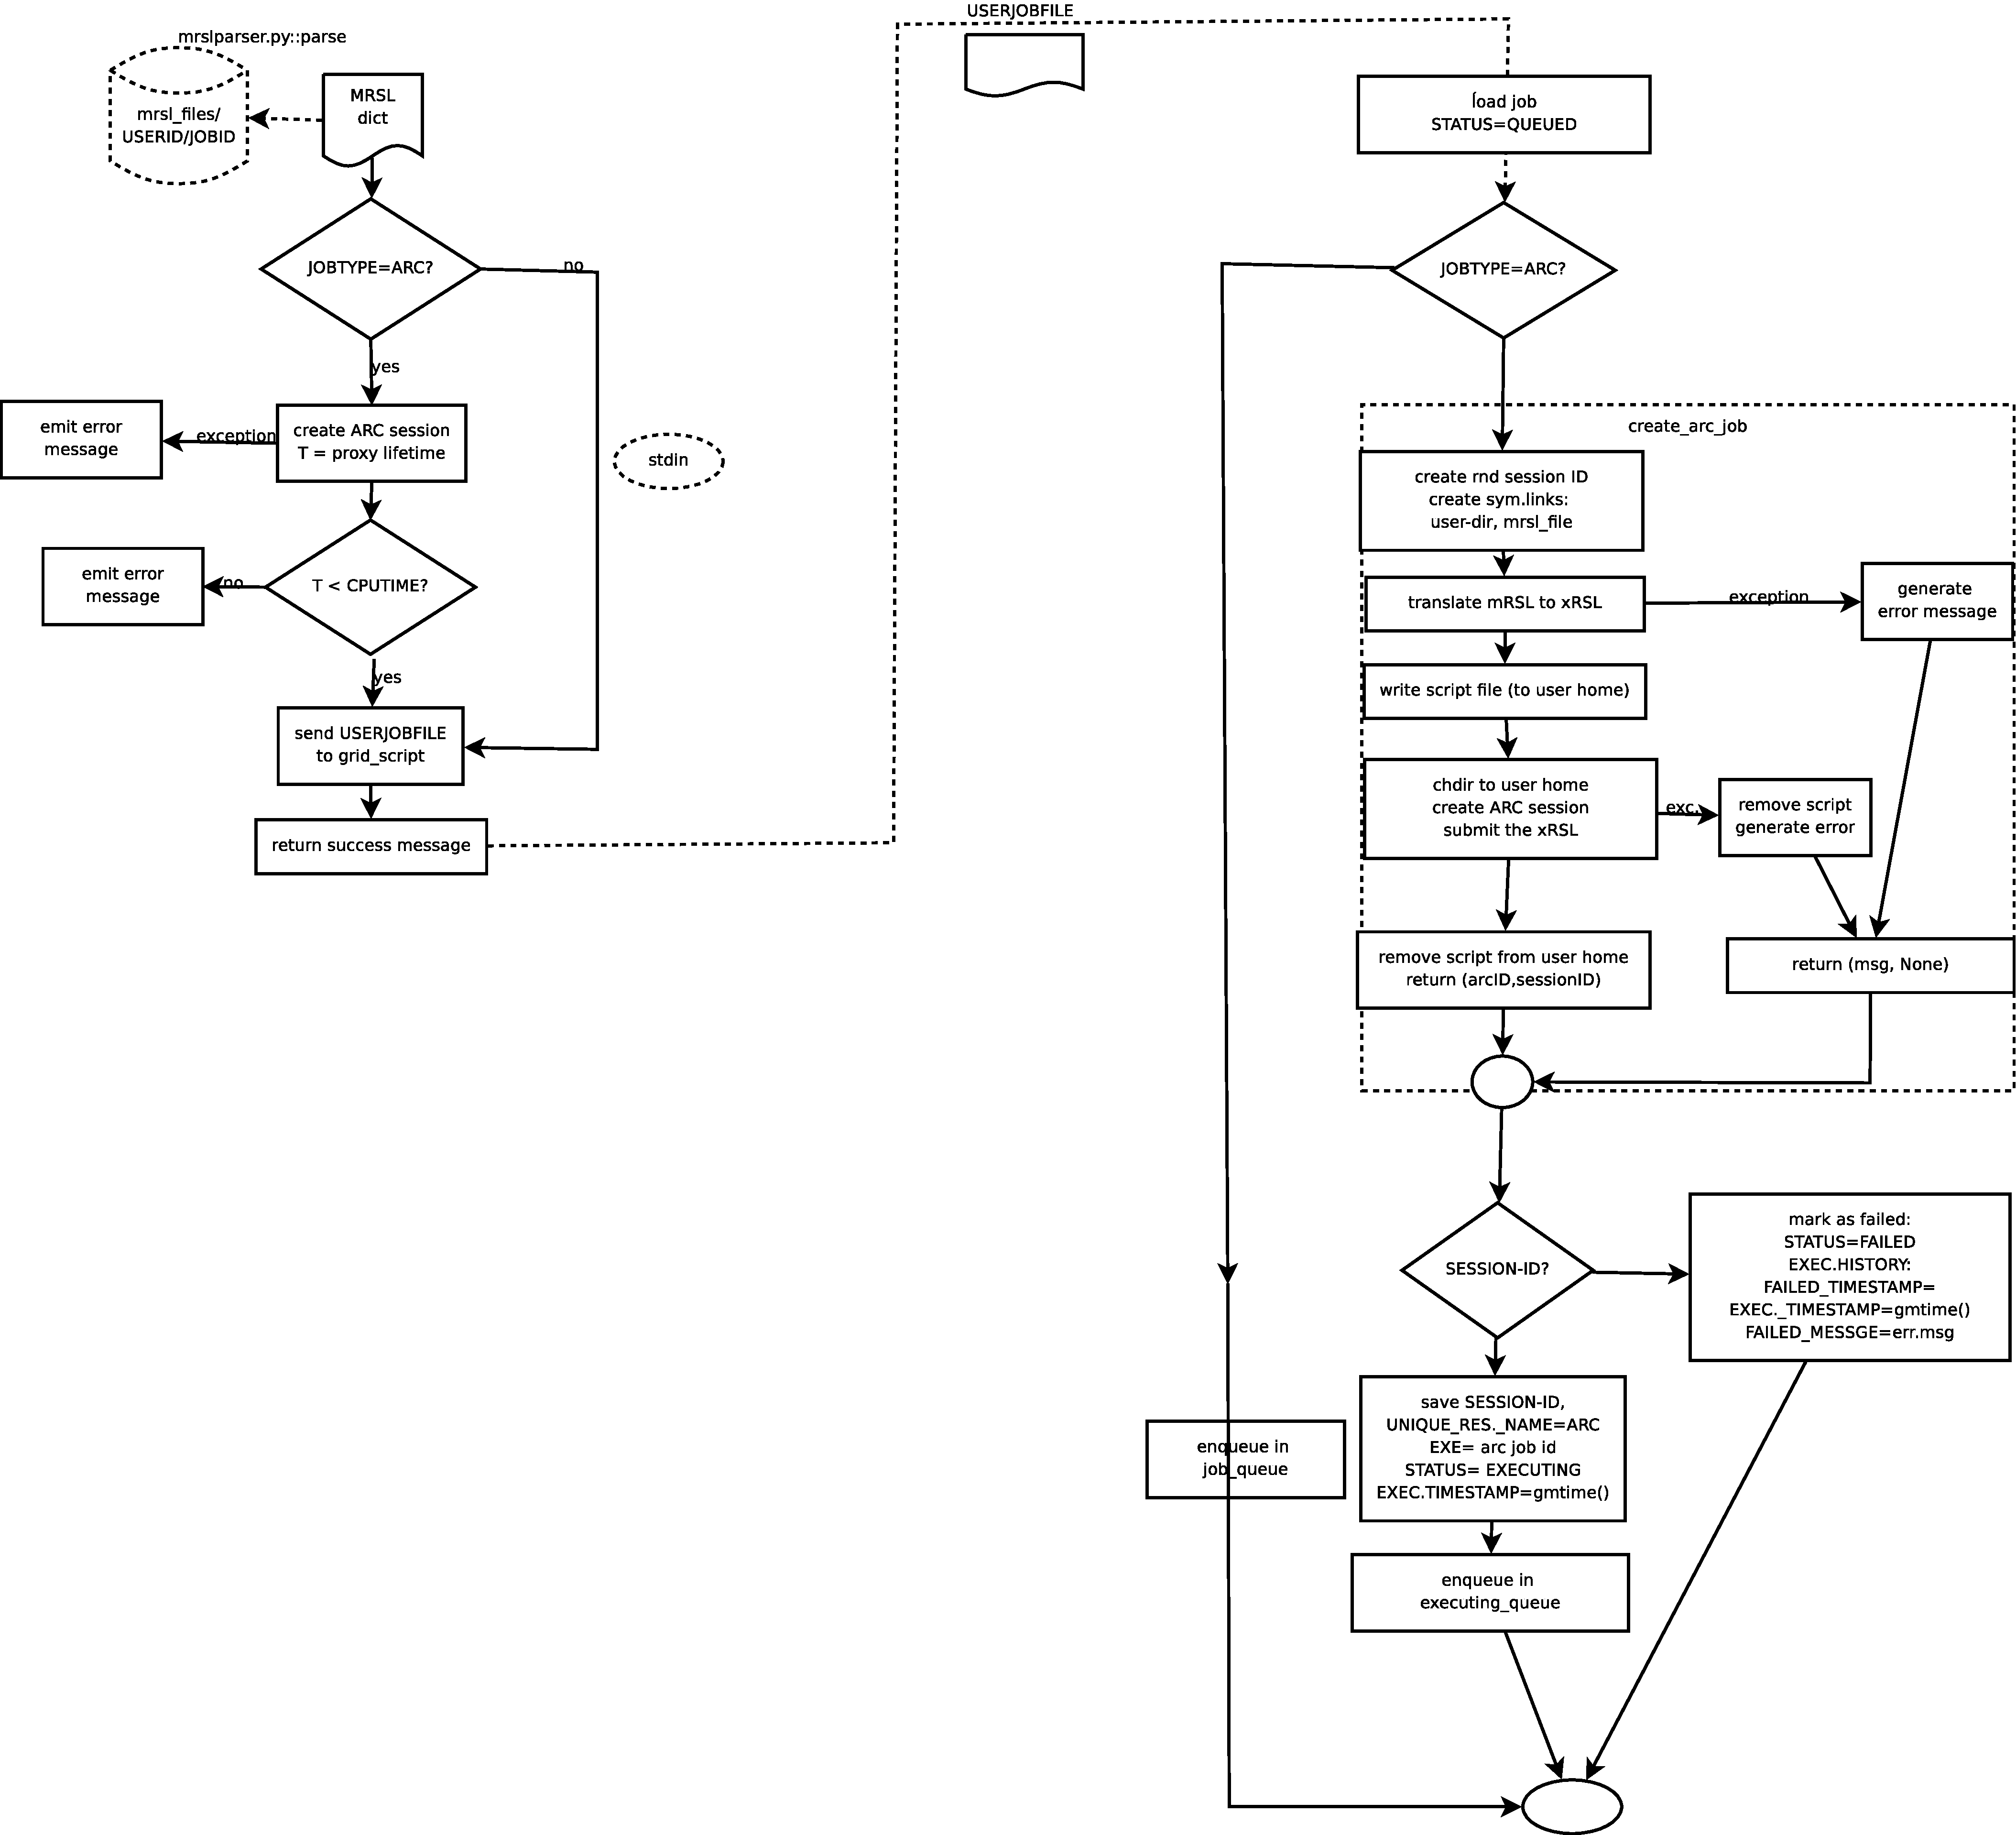
\includegraphics[height=0.6\textheight]{ARCsubmit}
\caption{ARC job submission from user and grid\_script}
\label{ARCsubmit}
\end{figure}

\verb!grid_script! will call this method and set the job status
according to the result: FAILED with error message, or EXECUTING (as
the default action). If submission fails, it creates an
EXECUTION\_HISTORY (expected by job status) and drops the job. If the
job is submitted, it saves the SESSION\_ID, ``ARC'' as field
UNIQUE\_RESOURCE\_NAME , and the ARC Job ID as field EXE.

\paragraph{Automatic transfer of results/output files:}
 In the prototype, specified output files, as well as stdout and
 stderr were retrieved by a request from the user. This is now
 done automatically, by adding https output destinations when not
 specified by the user. 

 Job output (split into stdout and stderr) will always be uploaded to
 the server, into a special directory \verb!job_output!. Other files
 are uploaded to a location relative to the user's home directory if
 no destination is specified (files can be renamed when
 uploading). Upload of directories is not supported (neither in ARC,
 nor in MiG).

 Technically, we use the same mechanism as existing MiG resources: inside
 \texttt{state/webserver\_home/}, a symbolic link to the (previously
 created) job output directory is created. The random name of this
 link acts as a session ID (since uploads are not
 authenticated). Session ID is generated and used when translating
 mRSL into xRSL, links are created and the job is submitted immediately.

\paragraph{Job Cleanup:}
 Cleanup for a job in MiG is usually triggered when a file with name
 \verb!*.status! is uploaded. For ARC jobs, we cannot presume a
 particular order of upload and thus have to do the cleanup separately
 (from grid\_script on a regular basis).

 
 We identify files coming from ARC by a missing (link to a) job file.
 Uploaded ARC files are simply stored inside their destination file,
 and no cleanup is triggered. Instead, the job timeout thread
 regularly requests the status of executing ARC jobs (jobs in the
 executing queue).  If the update yields status \verb!FINISHED!, the
 job is cleaned up directly.  (Instead, we could send a
 RESOURCEFINISHEDJOB event to grid\_script, but which turns out to be
 more complicated). 

 The updated status will \emph{not} be written into the job's mRSL
 file, see below.

\verb!grid_script! will handle ARC jobs a special case (this time
based on UNIQUE\_RESOURCE\_NAME = ARC, which allows future
extensions).  Cleaning up the job remainder is slightly different from
normal jobs (removing only two symbolic links, but cleaning it on the
ARC resource). The job also needs to be removed from the executing
queue.  Cleanup functionality, except accessing the executing queue,
is implemented as a helper function.


\paragraph{Job Status}
 MiG assumes that jobs handed out to resources are immediately
 executing. This is not true for the ARC variant, where jobs stay in a
 local queue. \jost{How does the PBS and SGE variant handle this,
   BTW?}

 The job status for MiG jobs is usually retrieved from the mRSL files
 (i.e. includes all historic data for finished jobs). ARC jobs have
 correct status in the mRSL file if they are finished, failed, or
 canceled. For ARC jobs with status ``executing'', the job status will
 be requested from ARC on request (Background: The MiG server does not
 use the mRSL file, but the dynamic data in the executing queue for
 all activities. Job status uses the mRSL, so these files would need
 regular update otherwise).

\paragraph{Job Timeout and Cancel:}
 \verb!grid_script! puts the job in the executing queue, so it will be
 checked by the timeout thread. The latter will send a message to the
 main server loop when jobs reach their timeout. Canceling a job
 works in the same way: a message is sent to the \verb!grid_script!,
 and the job will be removed from there.
 
\paragraph{Resource Information and Runtime Environments}

In the first version, no resource information for ARC resources is
given, and the implementation uses the available runtime environments
only implicitly (inside ARC brokering). In later versions, ARC
resources should be handled as resources of a special (sub-)VGrid, in
order to match the requested runtime environment beforehand. This
sub-VGrid can act as the current JOBTYPE flag.

\end{document}
